%%%%%%
%
% $Autor: Sudeshna Nanda $
% $Date: 2025-01-15 $
% $File name:  ProjectPresentation.tex
% $Version: 1.0 $
%
% !TeX encoding = utf8
%
%%%%%%
\section{Results}
\begin{frame}{Display Results}
	\begin{figure}[h]
		\centering
		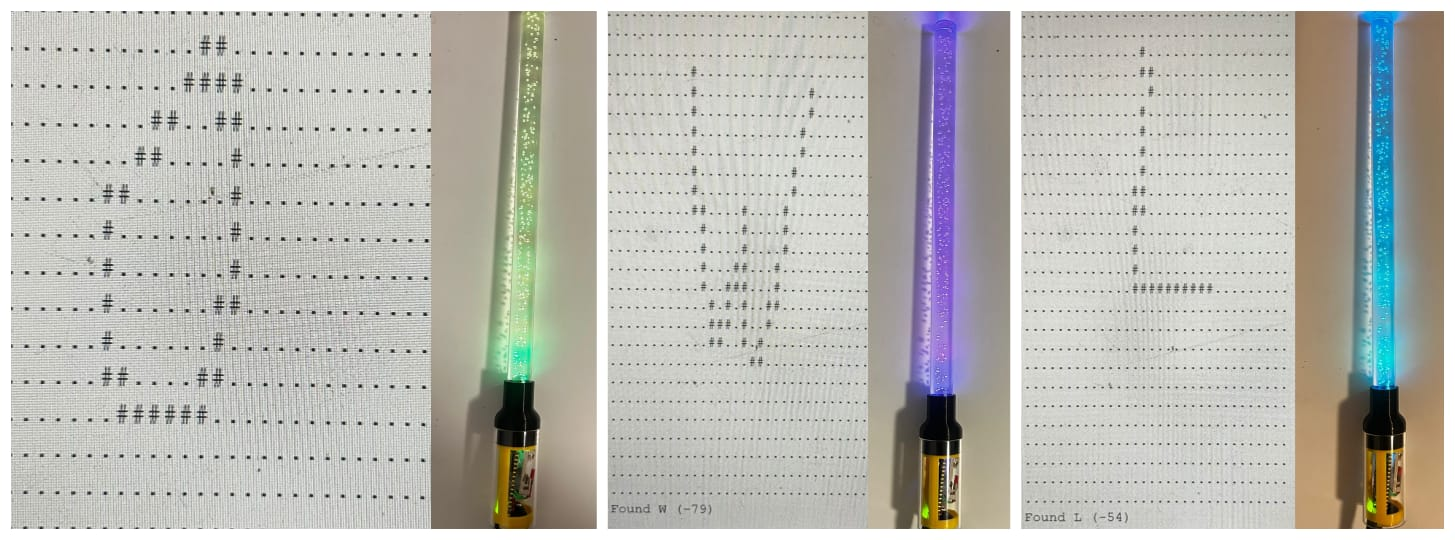
\includegraphics[width=\linewidth]{C:/Users/sudes/Documents/GitHub/ML24-06-Magic-Wand-with-an-Arduino-Nano-33-BLE-Sense/Presentations/MagicWand/img/MagicWandResults.jpeg}
		\caption{Magic Wand Results}
		\label{fig:magicwand_results}
	\end{figure}
	
\end{frame}


\begin{frame}{Results}

\textbf{Technical Achievements}
	\begin{itemize}
		\item Deployed a gesture-recognition system on the Arduino Nano 33 BLE Sense[\cite{Arduino:2015}].
		\item Used Convolutional Neural Networks (CNNs) for feature extraction and classification.
		\item Optimized model size and computational efficiency through quantization and pruning.
		\item Achieved real-time gesture recognition on edge devices.
	\end{itemize}



\textbf{Future Improvements}
	\begin{itemize}
		\item \textbf{Model Optimization:} Explore advanced pruning and quantization techniques[\cite{Shi:2016}].
		\item \textbf{System Robustness:} Enhance error handling for sensor data inconsistencies.
		\item \textbf{Scalability:} Recognize more gestures and integrate with additional applications.
		\item \textbf{User Experience:} Refine gesture output and response mechanisms.
	\end{itemize}
\end{frame}
